\newcommand\invisiblesection[1]{%
  \refstepcounter{section}%
  \addcontentsline{toc}{section}{\protect\numberline{\thesection}#1}%
  \sectionmark{#1}}

\externaldocument{chapter1}
\chapter{Introduction}
\label{Introduction1}
\invisiblesection{Preliminaries}
%This chapter includes motivation for the research study followed by the problems in random testing, the alternative approaches to overcome these problems, the research objectives and contributions of the study. At the end of the chapter, the structure of the remaining thesis is given.
%\section{Motivation} %In recent years there has been a particular increase in performing automated random testing and, specifically, the techniques for automatic generation of fault targeting test data. 
%Computer processors execute instructions composing programs designed and created by programmers. The set of all such machine readable instructions of a system is called software. This includes human-understandable instructions (source code) as well as machine-understandable instructions (binary code). Software is often written in high level languages that are close to natural language and are generally portable to multiple architectures. These languages require compiler or interpreter to transform them into an architecture specific, machine language before execution. 

%Software is an important and essential component of computer system without which no task can be accomplished. 
%software consists of clearly defined instructions that upon execution, instructs hardware to perform the tasks for which it is designed
Software is a set of clearly defined instructions for computer hardware to perform a particular task. Some software are developed for use in simple day to day operations while others are for highly complex processes in specialised fields like education, business, finance, health, science and technology etc. The ever increasing dependency on software tend us to believe that software are reliable, robust, safe and secure. Like every other man-made items software are also prone to errors. Maurice Wilkes~\cite{wilkes1985memoirs}, a British computer pioneer stated that,
\smallskip
\begin{quote}
``As soon as we started programming, we found to our surprise that it was not as easy to get programs right as we had thought. Debugging had to be discovered. I can remember the exact instant when I realized that a large part of my life from then on was going to be spent in finding mistakes in my own programs."
\end{quote}
\bigskip
The margin of error in mission-critical and safety-critical systems is so small that a minor fault can lead to large economic losses~\cite{huang2004securing}. According to the National Institute of Standards and Technology, US companies alone bear \$59.5 billion loss every year due to software failures, and that improvements in software testing infrastructure might save one-third of this cost~\cite{tassey2002economic}. Software testing is the most recognized and widely used technique to verify correctness and ensure quality of the software~\cite{patton2001software}. Therefore, software companies leave no stone unturned to ensure the reliability and accuracy of the software before its practical application. According to Myers et al. some software companies spend up to 50\% of the elapsed time and more than 50\% of the total development and maintenance cost on software testing~\cite{beizer2003software}. The success of a software testing technique mainly depends on the number of faults discovered in the SUT. An efficient testing process discovers maximum number of faults in minimum possible time. There is therefore a strong motivation for improving the existing strategies and developing new efficient test strategies. This research study is a contribution to the literature on the subject with the aim to bring about improvement in software testing by devising new and improved automated software testing techniques based on random strategy.

Ideally exhaustive testing, where software is tested against all possible inputs, may look more attractive but it is commonly not feasible because of large size of input domain, limited resources and strict time constraints. The usual practice is therefore to use a test strategy for the selection of test data set from a large/infinite domain. Careful selection of the test data set, as a subset of the whole input domain, is a crucial factor in any testing technique because it represents the whole domain for evaluating the structural and/or functional properties of the SUT~\cite{howden1986functional, mccabe1983structured}. Miller and Maloney were the first who comprehensively described a systematic approach of test data set selection known as path coverage. They proposed that testers should select the test data set so that all paths of the SUT are executed at least once~\cite{miller1963systematic}. The approach resulted in higher standard of test quality. %A large number of test strategies were subsequently developed such as boundary value analysis and equivalence class. 

Test data set can either be generated manually or automatically. Generating test data set manually is a time-consuming and laborious exercise~\cite{korel1990automated} as compared to the more preferable automated test data set generation. Test data generators can be of different types i.e. Path-wise (Section~\ref{sec:pathwise_2}), Goal-oriented (Section~\ref{sec:goaloriented_2}), Intelligent (Section~\ref{sec:intelligent_2}), search-based (Section~\ref{sec:search_based_2}) and Random (Section~\ref{sec:randomgenerator_2}).

Based on the critical importance of relevant test data set, the testers should always use the most efficient test strategy during software testing. However, using such a test strategy involves higher cost to generate test data set that satisfy complex constraints requiring extra computation. Therefore an optimum approach is desired to maintain a balance between the resources required and the generation of relevant test data set to make the software testing cost effective. Random test data set generation approach is simple, widely applicable, easy to implement, faster in computation, free from bias and costs minimum overhead~\cite{ciupa2007experimental}. Its effectiveness can be further increased by slight alteration in its algorithm~\cite{chen2005adaptive}.


%The process of evaluating the correctness and quality of the software or its component is called software testing. 

%Software is a very important and essential component of computer system without which no task can be accomplished. Some softwares are developed for use in simple day to day operations while others are for highly complex processes in specialized fields like research and education, business and finance, defence and security, health and medicine, science and technology, aeronautics and astronautics, commerce and industry, information and communication, environment and safety etc. The ever increasing dependency of software expect us to believe that the software in use is reliable, robust, safe and secure. Unfortunately, the performance of software in general is not what is expected. According to the National Institute of Standards and Technology (NIST), US companies alone bear \$60 billion loss every year due to software failures and one-third of that can be eliminated by an improved testing infrastructure~\cite{Standards2002}. Humans are prone to errors and programmers are no exceptions. Maurice Wilkes~\cite{Maurice1985}, a British computer pioneer, stated that:
%\begin{quote}
%``As soon as we started programming, we found to our surprise that it was not as easy to get programs right as we had thought. Debugging had to be discovered. I can remember the exact instant when I realized that a large part of my life from then on was going to be spent in finding mistakes in my own programs."
%\end{quote}

%The margin of error in mission-critical and safety-critical systems is so small that a minor fault can lead to huge economic losses~\cite{huang2004securing}. Therefore, software companies leave no stone unturned to ensure the reliability and accuracy of the software. Software testing is by far the most recognized and widely used technique to verify the correctness and ensure quality of the software ~\cite{Standards2002, Myers2011, patton2001software, young2008software}.  According to Myers et al. some software companies spend up to 50\% cost of the total cost of software development and maintenance on testing~\cite{Myers2011}. 

\section{Software Testing} 
Software testing is a Verification and Validation (V\&V) technique used to ensure that the software adheres to the desired specifications. According to Edsger Dijkstra, software testing can be used to show the presence of bugs but never to show the absence of bugs~\cite{dahl1972structured}. It means that a software under test (SUT) that passes all the tests without giving any error is not guaranteed to contain no error. However, the testing process increases reliability and confidence of users in the tested product. Software testing is discussed in more detail in Section~\ref{sec:softwareTesting}.

 

\section{Random Testing} 
It is a testing technique in which test data set is randomly generated in accordance with the requirements, specifications or other test adequacy criteria. The given SUT is executed against the test data set and results obtained are evaluated to determine whether the output produced satisfies the expected results. According to Godefroid et al.~\cite{godefroid2005dart}, ``Random testing is a simple and well-known technique which can be remarkably effective in discovering software bugs". The three main phases of random testing include data generation, execution and evaluation as shown in Figure~\ref{fig:SoftwareTesting1}. Random testing is discussed in more detail in Section~\ref{sec:randomTesting}.
\bigskip
\bigskip
\begin{figure}[H]
	\centering
		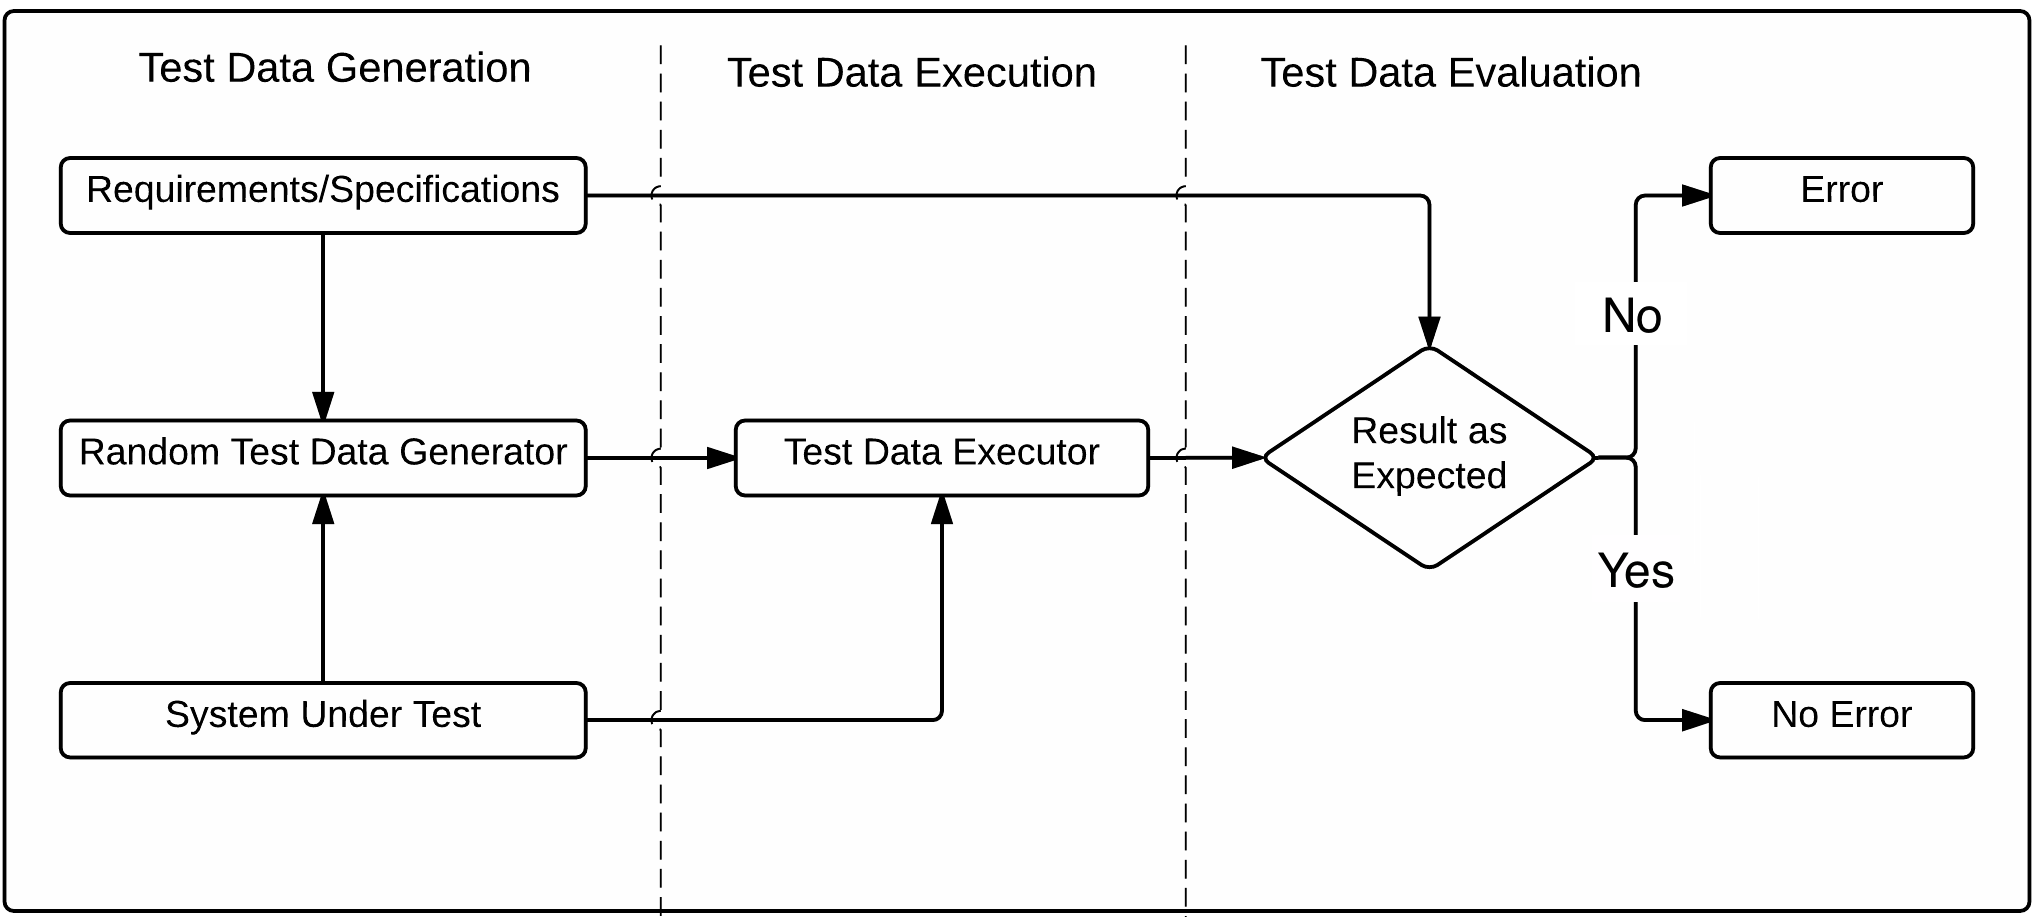
\includegraphics[width=15.3cm, height=7cm ]{chapter1/randomTestingPhases1.png}
		\caption{Three main phases of random testing}
	\label{fig:SoftwareTesting1}
\end{figure}
\bigskip
\textbf{Test Data Generation:} It includes generation/selection of test data set for use as input to the SUT. In this phase the tester is free to generate test data set arbitrarily from the input domain without any test adequacy criteria. Nevertheless, the two most commonly used methods are uniform distribution and operational profile. In uniform distribution all inputs are equally probable for selection. In operational profile the test data are selected as if the program under test is used in operational environment.

\textbf{Test Data Execution:} It includes application of the generated test data set to the SUT. The process consists of three steps: supplying test data as input to the software, executing the software and logging the output obtained. 
These steps can be achieved manually by hand or automatically by using a script or tool. 
%to save time and facilitate repetition.

\textbf{Test Data Evaluation:} It includes analysis of the test logs to know whether the test is fail or pass. The decision of fail/pass is made by comparing the obtained results with the correct results contained in the test oracle. The data evaluation can be performed either manually or automatically.

%

\section{The Problems}
Despite the benefits of random testing, its simplistic and non-systematic nature exposes it to high criticism~\cite{myers2011art, white1987software}. This research study focuses on the following problems in automated Random Testing (RT):
%Myers et al.~\cite{myers2011art} mentioned, ``probably the poorest methodology of all is random-input testing".  Despite the benefits of random testing, its simplistic and non-systematic nature exposes it to high criticism~\cite{white1987software}. Myers et al.~\cite{myers2011art} mentioned, ``probably the poorest methodology of all is random-input testing". However, Ciupa et al.~\cite{ciupa2008artoo} reported that the above stated statement of Myers et al. is based on intuition and lacks any experimental evidence. The criticism motivated the researchers to look into various aspects of random testing for evaluation and possible improvement. Adaptive random testing (ART)~\cite{chen2005adaptive}, Restricted Random Testing (RRT)~\cite{chan2006restricted}, Feedback Directed Random Testing (FDRT)~\cite{pacheco2007randoop}, Mirror Adaptive Random Testing (MART)~\cite{chen2004mirror} and Quasi Random Testing (QRT)~\cite{chen2007quasi} are a few of the enhanced random testing techniques reported in the literature.


\begin{enumerate}
\item Limitation of RT to discover contiguous failures.
\item Inability of RT to identify failure-domains.
\item Incompetence of RT to present results in graphical form. 
\end{enumerate}

\subsection{Limitation of RT to discover contiguous failures}
Chan et al.~\cite{chan1996proportional} observed that failure inducing inputs are contiguous and form certain geometrical patterns in the whole input domain. They divided them into point, block and strip domains on the basis of their shape (Section~\ref{sec:failuredomains_2}). % put the failure domains section label in the preceeding reference.
The failure-finding ability of random testing technique is quite low to detect the contiguous block and strip failure domains within the input domain. Attempts are needed to overcome this limitation of RT by developing a suitable extended random strategy.

\subsection{Inability of RT to Identify Failure-domains}
%As stated above, the failures in the input domain are contiguous and form point, block and strip patterns. 
Majority of failures reside in contiguous locations and form certain failure domains across the input domain~\cite{chan1996proportional}. The existing random strategies of software testing tries to discover failures individually from the domains and lack the capability to discover the failure-domains. Endeavours are required to be undertaken for developing appropriate random strategy with the potential to identify the failures as well as failure-domains. 

%Random testing is also considered weak in providing high code coverage~\cite{cohen1997aetg, offutt1996semantic}. For example, in random testing when the conditional statement  ``$if (x == 25) then ... $"  is exposed to execution then there is only one chance, of the ``$then...$" part of the statement, to be executed out of $2^\text{32}$ available options. If $x$ is an integer variable of 32 bit value~\cite{godefroid2005dart}. 

\subsection{Incompetence of RT to Present Results in Graphical Form}
Random testing is no exception when it comes to the complexity of understanding and evaluating test results. Modern testing techniques simplify results by truncating the lengthy log files and displaying only the fault revealing test cases in the form of unit tests. No random strategy seems to provide graphical representation of the failures and failure-domains. Efforts are therefore required to get the test results of random testing in user-friendly graphical form in addition to the textual form. 

%\subsection{To study the nature of Failure domain}





\section{Research Goals}\label{ResearchGoals_1}
Research goals of the current study are: to understand the nature of failures, to leverage failure domain for finding more bugs, to develop new improved automated random strategies.

%Goals of the research study are discovering how to leverage failure domain for finding more bugs and understanding the nature of failures and to develop new improved automated random test strategies to achieve the desired goals.

%The main goal of the research study is to develop new techniques for automated random testing with the aim to achieve the following objectives:

%\begin{enumerate}
%\item To develop a testing strategy with the capability to generate more fault-finding test data.

%\item To develop a testing technique for finding faults, fault domains and presentation of results on a graphical chart within the specified lower and upper bound. 

%\item To develop a testing framework with focus on increase in code coverage along with generation of more fault-finding test data. 

%\end{enumerate}

\section{Contributions}\label{contributions_1}
The main contributions of the thesis research are as follows: 

\subsection{Dirt Spot Sweeping Random Strategy}
%Development of a new enhanced and improved form of automated random testing: the Dirt Spot Sweeping Random (DSSR) strategy. This strategy is based on the assumption that faults and unique failures reside in contiguous blocks and stripes. The DSSR strategy starts as a regular random+ testing strategy � a random testing technique with preference for boundary values. When a failure is found, it increases the chances of using neighbouring values of the failure in subsequent tests, thus slowly sweeping values around the failures found in hope of finding failures of different kind in its vicinity.
%The DSSR strategy is implemented in the YETI random testing tool. It is evaluated against random (R) and random+ (R+) strategies by testing 60 classes (35,785 line of code) with one million ($10^\text{6}$) calls for each session, 30 times for each strategy. The results indicate that for 31 classes, all three strategies find the same unique failures. We analysed the 29 remaining classes using t-tests and found that for 7 classes DSSR is significantly better than both R+ and R, for 8 classes it performs similarly to R+ and is significantly better than R, and for 2 classes it performs similarly to random and is better than R+. In all other cases, DSSR, R+ and R do not perform significantly differently. Numerically, the DSSR strategy finds 43 more unique failures than R and 12 more unique failures than R+.

The failure-finding ability of random testing technique decreases when the failures lie in contiguous locations across the input domain. Dirt Spot Sweeping Random (DSSR) strategy was developed as a new automated technique to overcome the problem. It is based on the assumption that unique failures reside in contiguous blocks and strips. When a failure is identified, the DSSR strategy selects neighbouring values for the subsequent tests. The selected values sweep around the failure, leading to the discovery of new failures in the vicinity. Results presented in Chapter~\ref{chap:DSSR} indicate higher failure-finding ability of DSSR strategy as compared with Random and Random+ strategies.

\subsection{Automated Discovery of Failure Domain}
The existing random strategies of software testing discover the failures in the SUT but lack the capability of presenting the failure domains. In the present study, a fully automated testing strategy named, ``Automated Discovery of Failure Domain (ADFD)" is developed with the ability to find failures as well as failure domains in a given SUT and provides visualisation of the identified pass and fail domains in a graphical form. The strategy implemented in YETI is described and practically illustrated by executing several programs of one and two dimensions in Chapter~\ref{chap:ADFD}. The experimental results provide evidence that the newly developed ADFD strategy performs identification of failures as well as failure-domains and provides the results in graphical form.

\subsection{Automated Discovery of Failure Domain+}
Automated Discovery of Failure Domain+ (ADFD+) is an upgraded version of ADFD technique with respect to algorithm and graphical representation of failure-domains. The new algorithm searches for the failure-domain around the failure in a given radius as against ADFD which limits the search between lower and upper bounds. In addition, ADFD output is improved to provide labelled graphs which make ADFD+ output easily understandable and user friendly. ADFD+ is compared with an automated testing tool Randoop to find the comparative performance of the two techniques on similar programs. The results in Chapter~\ref{chap:ADFD+} indicated that in comparison with Randoop, its efficiency is evident by taking two orders of magnitude less time and its effectiveness is shown by taking 50\% or less number of test cases to discover failure domains.


\subsection{Evaluation of ADFD and ADFD+ using Qualitas Corpus}
An experimental evaluation of ADFD and ADFD+ techniques to measure their effectiveness in revealing failure-domains. The analysis of comparative performance of automated techniques with manual technique. The subject programs include open source packages included in the Qualitas Corpus.


%ADFD+ has the added advantage of presenting the output in graphical form showing point, block and strip domains visually as against Randoop, which lacks graphical user interface.



%To find the effectiveness of ADFD+, it was compared with Daikon by using error seeded programs. The ADFD+ correctly pointed out all the seeded failure domains while Daikon identified individual failures but was unable to discover the failure domains.

%IGRS is an extended form of Random+ strategy guided by software invariants. Invariants from the given SUT are collected by Daikon, filtered by using DynComp and annotated in to source code as assertions. The IGRS is implemented in YETI and generates values in compliance with the added assertions. Experimental results presented in Chapter~\ref{chap:ADFD+} indicate improved features of IGRS in terms of higher code coverage and identification of subtle errors that R, R+ and DSSR strategies are either unable to accomplish or require larger duration.  

%\section{Structure of the Thesis}
%
%The rest of the thesis is organized as follows: In Chapter 2, a thorough review of the relevant literature is given. It includes a brief introduction of software testing techniques followed by automated random testing tools. Chapter~\ref{chap:DSSR} describes Dirt Spot Sweeping Random (DSSR) strategy, which is based on sweeping of fault clusters in the input domain. Chapter~\ref{chap:ADFD} presents the newly developed Automated Discovery of Fault Domains  (ADFD) strategy, which focuses on dynamically finding the faults and domains along with their graphical representation. Chapter~\ref{chap:IGR+S} presents the new strategy Invariant Guided Random+ Strategy (IGR+S) developed with the focus on quick identification of faults and increase in code coverage with the help of assertions. Chapter 6 summarizes contributions of the thesis research, discusses the strength and weaknesses of the study, gives conclusion and suggests avenues for future work. Chapter 7 ?
\bigskip
\section{Structure of the Thesis}

The rest of the thesis is organized as follows:\\

\hangindent=\parindent
\hangafter=1
\noindent
\textbf{Chapter~\ref{chap:softwareTesting}} provides literature review on software testing. Software testing is introduced with particular reference to its level, purpose, perspective and execution. Various types of software testing followed by major stages of testing including test data generation, execution, oracle and report production are reviewed with particular focus on literature relevant to random testing. Various versions of random testing and the most commonly used automated testing tools based on random algorithms are reviewed. \\


\hangindent=\parindent
\hangafter=1
\noindent
\textbf{Chapter~\ref{chap:yeti_3}} presents the York Extensible Testing Infrastructure (YETI), used as a tool in our experiments. YETI has been thoroughly reviewed including an overview, design, core infrastructure, strategy, language-specific binding, construction of test cases, command line options, execution, test oracle, report generation and graphical user interface.\\

\hangindent=\parindent
\hangafter=1
\noindent
\textbf{Chapter~\ref{chap:DSSR}} describes the Dirt Spot Sweeping Random (DSSR) strategy. The proposed new testing technique is implemented in YETI. Experimental evidence is presented in support of the effectiveness of DSSR strategy in finding failures and failure domains as compared with random and random+ strategies. \\
% In majority of the classes DSSR strategy indicates higher fault-finding ability than random and random+ strategies. \\

\hangindent=\parindent
\hangafter=1
\noindent
\textbf{Chapter~\ref{chap:ADFD}} presents Automated Discovery of Failure Domain (ADFD) strategy. The proposed new testing technique, implemented in YETI, finds failures and failure domains in a specified limit and plots them on a chart. Experimental evidence is presented in support of ADFD strategy applied to several one and two dimensional programs. \\

 
\hangindent=\parindent
\hangafter=1
\noindent
\textbf{Chapter~\ref{chap:ADFD+}} presents the Automated Discovery of Failure Domain+ (ADFD+) strategy. It is an upgraded version of ADFD technique with respect to algorithm and graphical representation of failure domains. To find the effectiveness of ADFD+, it was compared with Daikon using error seeded programs and the results are reported.\\ 


%Automated Discovery of Failure Domain+ (ADFD+) is an upgraded version of ADFD technique with respect to algorithm and graphical representation of failure domains. To find the effectiveness of ADFD+, it was compared with Daikon using error seeded programs. The ADFD+ correctly pointed out all the seeded failure domains while Daikon identified individual failures but was unable to discover the failure domains.
%The IGRS technique like DSSR and ADFD is also implemented in YETI. Experimental study is presented in which the effectiveness of IGRS in finding faults is compared with the random, random+ and DSSR strategies. 
% For the majority of the classes IGRS indicated higher fault-finding ability than the rival strategies.\\
\hangindent=\parindent
\hangafter=1
\noindent
\textbf{Chapter~\ref{chap:Evaluation}} presents the extensive experimental analysis of Java projects contained in Qualitas Corpus for finding the effectiveness of automated techniques (ADFD and ADFD+). The results obtained were analysed and cross-checked using manual testing. The impact of nature, location, size, type and complexity of failure-domains on the testing techniques were studied. \\

\hangindent=\parindent
\hangafter=1
\noindent
\textbf{Chapter~\ref{chap:conclusions_8}} provides conclusions of the study including contributions and the lessons learned.\\

\hangindent=\parindent
\hangafter=1
\noindent
\textbf{Chapter~\ref{chap:futureWork}} highlights the opportunities for future work, challenges that may be faced and possible approaches to overcome the challenges.\\


 \hangindent=\parindent
 \hangafter=1
 \noindent
 \textbf{Appendix~\ref{chap:appendix1}} includes ADFD logic implementation and Java programs with point, block and strip failure domains.\\

\newpage
\begin{figure}[h]
	\centering
		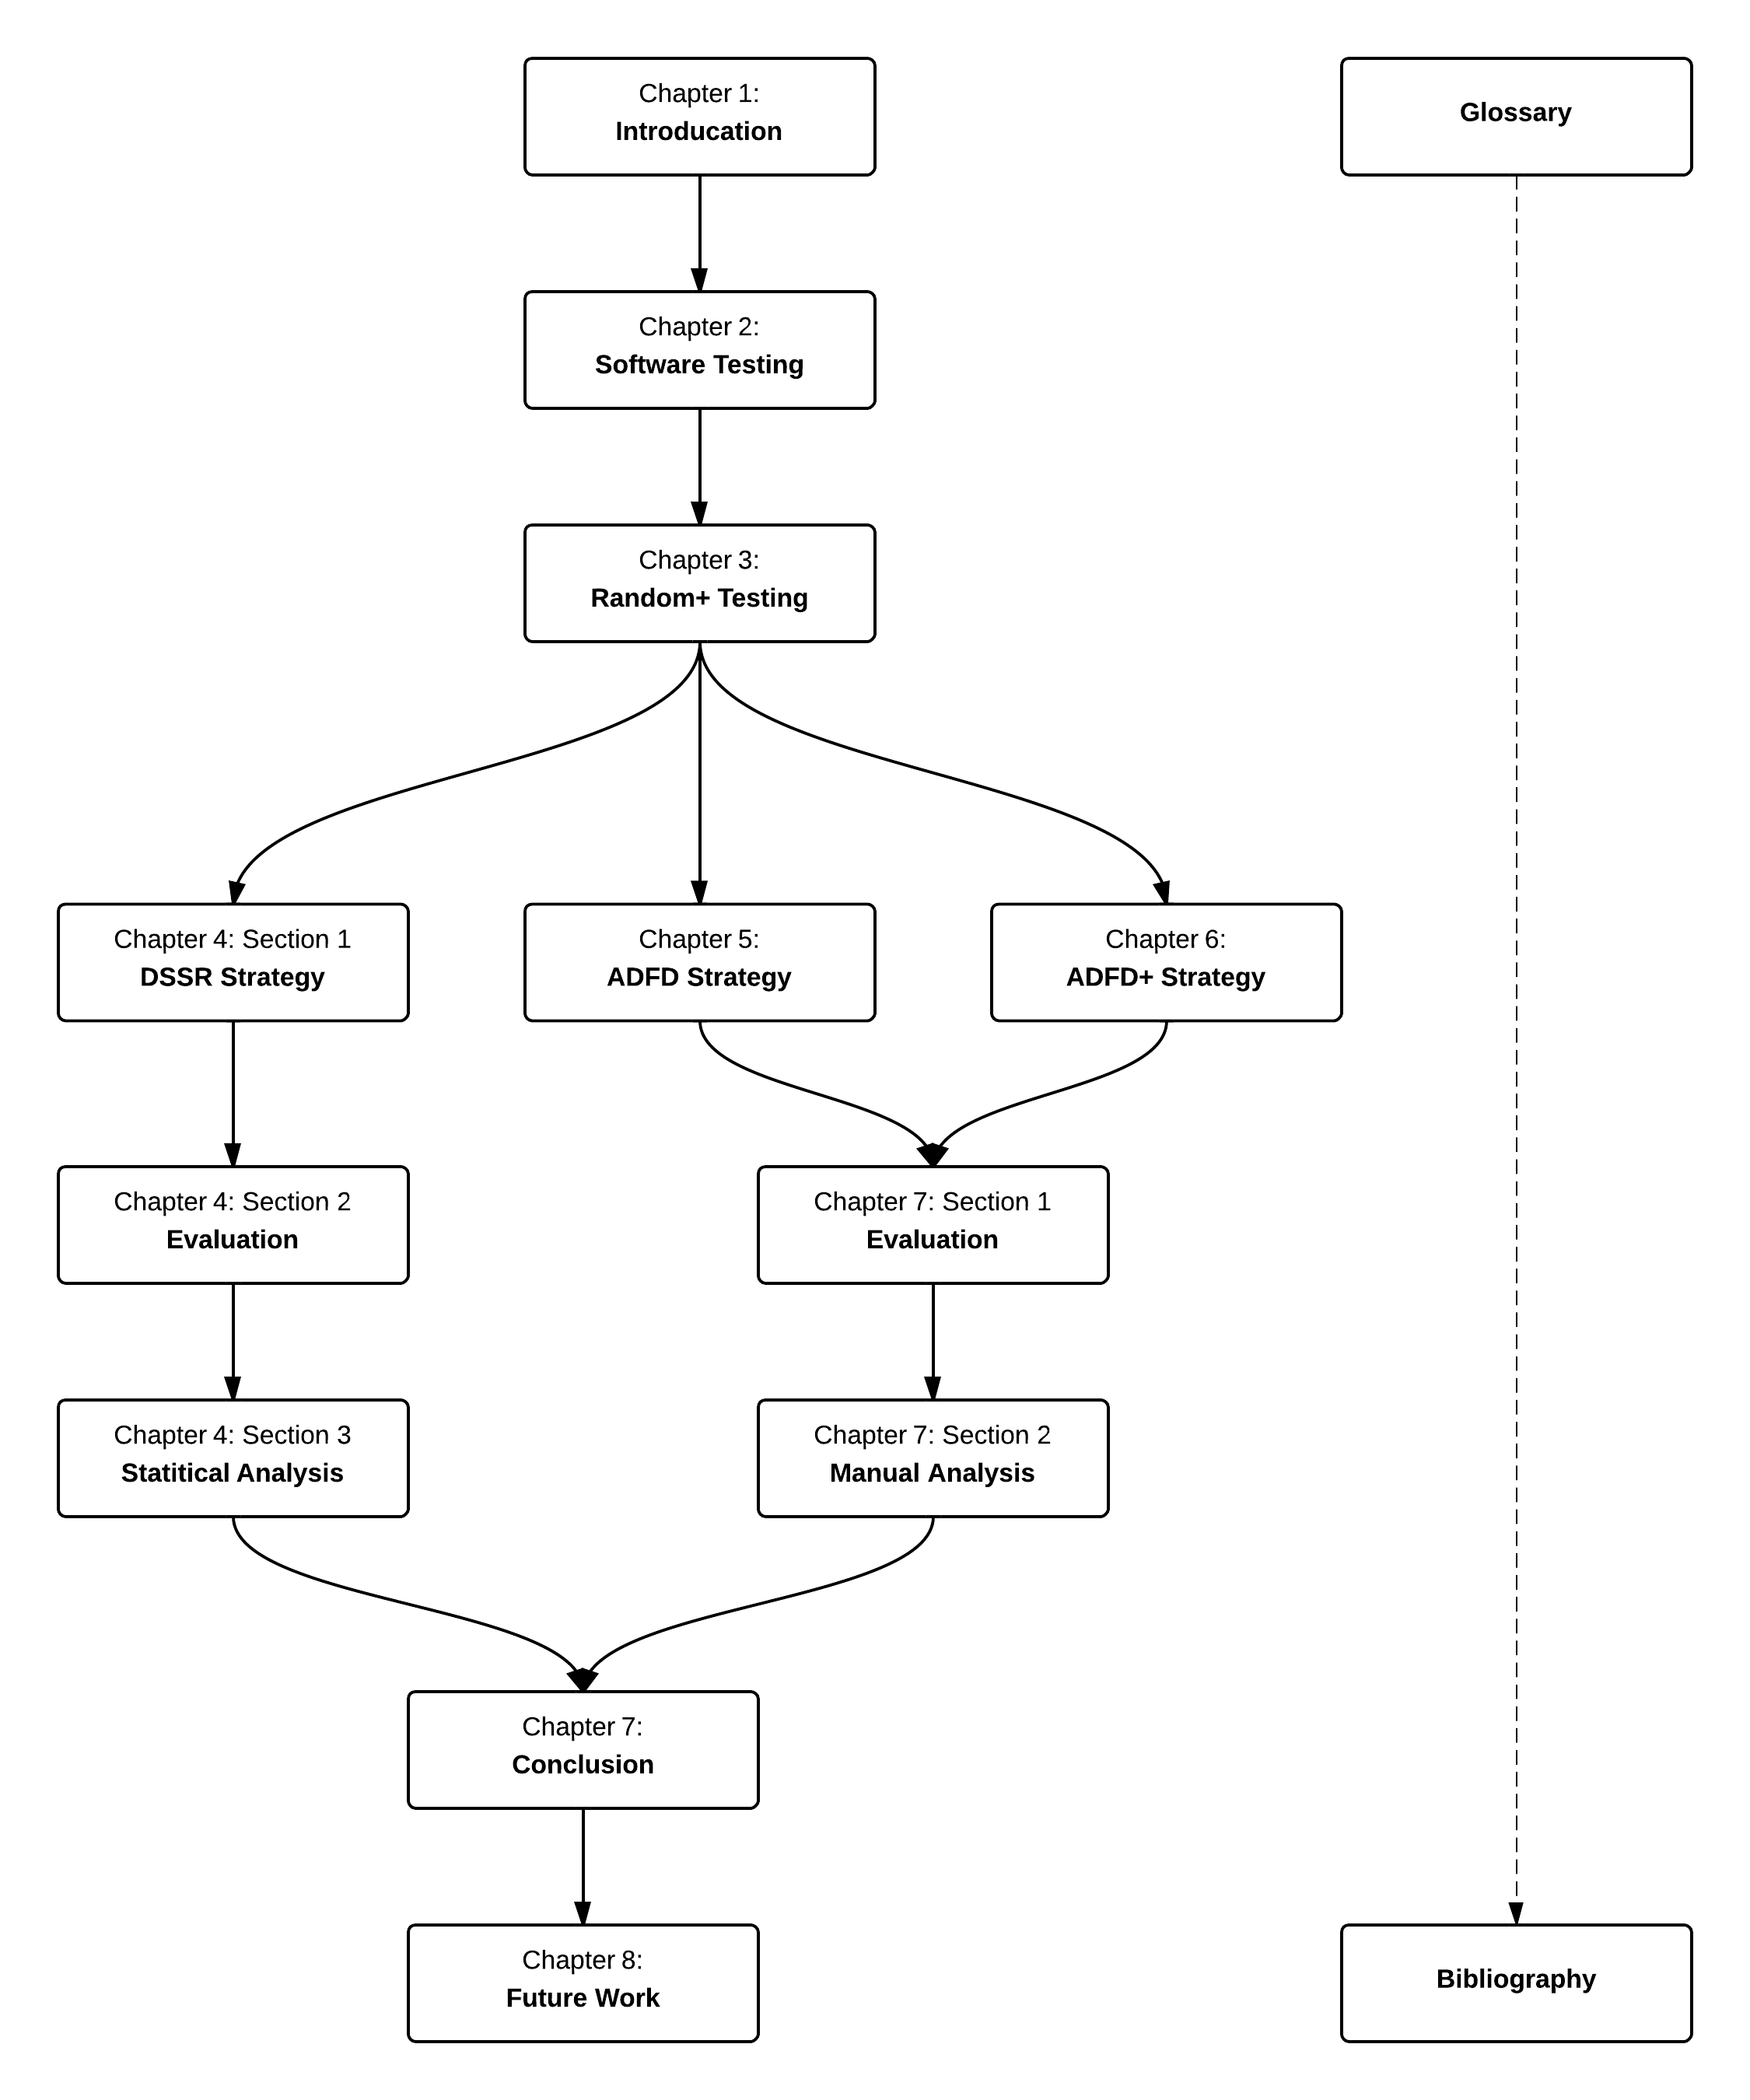
\includegraphics[width=16cm, height=20cm ]{chapter1/thesisOutline2.png}
		\bigskip
		\caption{Structure of thesis outline}
	\label{fig:thesisOutline}
\end{figure}



%Today, the primary focus of software companies is to achieve high quality. These companies spend an estimated thirty to ninety percent of the total software development cost on testing \ref{Beizer1990}, \ref{Standards2002}. In spite of spending 

%Software testing is the process of executing a software with specific test data followed by evaluation of the results to check whether it is working according to its specification or not \ref{Sommerville2006}.
% check here if we can replace specification with oracle or not.
%The test passes if the output complies to its specification and fails otherwise. The success of testing correlates with the number of failures found in the Software Under Test (SUT): a test is more successful if it finds more faults.

%It is interesting that program testing is used to show the presence of bugs, rather than absence of bugs [6]. Therefore the SUT that passes all the tests without returning a single failure does not guarantee that there is no fault. The testing process increases however the reliability and confidence of both the developers and the users in the tested product [7] [8] [9].

%Random testing is a black-box testing technique in which the SUT is executed against ran- domly selected test data. Test results obtained are compared either against the oracle defined, using SUT specifications in the form of assertions or exceptions defined by the programming language. The rapid increase in software development in today?s modern world prompts the need for automated testing to ensure high quality. The generation of random test data is com- paratively cheap and does not require too much intellectual and computation efforts [10] [11]. It is for this reason that various researchers have recommended this strategy for incorporation in automatic testing tools [12]. YETI [13] [14], AutoTest [15] [16], QuickCheck [17], Randoop [18], JArtage [19] are a few of the most common tools based on random strategy.


%%% ----------------------------------------------------------------------


%%% Local Variables: 
%%% mode: latex
%%% TeX-master: "../thesis"
%%% End: 
